\documentclass[12pt, a4paper]{article}

% Required Packages
\usepackage[utf8]{inputenc}
\usepackage{amsmath}
\usepackage{amssymb}
\usepackage{tikz} % Crucial for drawing Hasse Diagrams
\usepackage[margin=1in]{geometry}
\usepackage{setspace}

\begin{document}

% --- TITLE PAGE ---
\begin{titlepage}
    \centering
    \vspace*{2cm}
    
    {\scshape\LARGE Mathematics for Computing\par}
    \vspace{0.5cm}
    {\scshape\Large Assignment 1\par}
    \vspace{0.5cm}
    
    \vspace{2cm}
    
    {\Large \textbf{Sidharth H}}\par
    \vspace{0.5cm}
    {\large M.Tech CSE (AI \& DS) - Semester 1}\par
    
    \vfill
    
    % Date
    {\large August 2026\par}
\end{titlepage}

\newpage
\tableofcontents
\newpage

\setstretch{1.25}

% --- SECTION 1: 10 SETS ---
\section{10 Sets in Mathematical Form}
Below are 10 standard examples of sets represented in mathematical notation:

\begin{enumerate}
    \item \textbf{Natural Numbers:} $\mathbb{N} = \{1, 2, 3, 4, \dots\}$
    \item \textbf{Whole Numbers:} $\mathbb{W} = \{0, 1, 2, 3, \dots\}$
    \item \textbf{Integers:} $\mathbb{Z} = \{\dots, -3, -2, -1, 0, 1, 2, 3, \dots\}$
    \item \textbf{Rational Numbers:} $\mathbb{Q} = \left\{ \frac{p}{q} \mid p, q \in \mathbb{Z}, q \neq 0 \right\}$
    \item \textbf{Real Numbers:} $\mathbb{R} = \{x \mid x \text{ is a rational or irrational number}\}$
    \item \textbf{Set of Even Integers:} $E = \{2n \mid n \in \mathbb{Z}\}$
    \item \textbf{Set of Odd Integers:} $O = \{2n + 1 \mid n \in \mathbb{Z}\}$
    \item \textbf{Set of Prime Numbers:} $P = \{x \in \mathbb{N} \mid x > 1 \text{ and the only divisors of } x \text{ are } 1 \text{ and } x\}$
    \item \textbf{Boolean Set:} $B = \{0, 1\}$
    \item \textbf{A Continuous Interval:} $I = \{x \in \mathbb{R} \mid 0 \le x \le 1\}$
\end{enumerate}

\vspace{0.5cm}

% --- SECTION 2: INCLUSION-EXCLUSION ---
\section{General Form of the Inclusion-Exclusion Principle}
The Inclusion-Exclusion Principle is a counting technique used to calculate the number of elements in a union of multiple sets by systematically adding and subtracting the sizes of their intersections.

For a finite number of sets $A_1, A_2, \dots, A_n$, the general mathematical form is given by:

\begin{align*}
    \left| \bigcup_{i=1}^n A_i \right| &= \sum_{i=1}^n |A_i| - \sum_{1 \le i < j \le n} |A_i \cap A_j| + \sum_{1 \le i < j < k \le n} |A_i \cap A_j \cap A_k| \\
    &\quad - \dots + (-1)^{n-1} |A_1 \cap A_2 \cap \dots \cap A_n|
\end{align*}

\vspace{0.5cm}

% --- SECTION 3: TYPES OF SETS (AI/DS EXAMPLES) ---
\section{Types of Sets with AI and Data Science Examples}
\begin{itemize}
    \item \textbf{Finite Set:} A set containing a countable number of elements. \\
    \textit{Example (AI/DS):} The set of predefined object classes detected by a YOLOv8 waste classification model deployed on an edge device: $W = \{\text{plastic}, \text{glass}, \text{metal}, \text{paper}\}$.
    
    \item \textbf{Infinite Set:} A set that contains an endless number of elements. \\
    \textit{Example (AI/DS):} The set of all possible continuous weight and bias updates generated during the training loop of a Generative Adversarial Network (GAN).
    
    \item \textbf{Empty (Null) Set ($\emptyset$):} A set containing no elements. \\
    \textit{Example (AI/DS):} The set of false positive bounding boxes generated by an object detection model that achieves perfect 100\% precision on a given test batch.
    
    \item \textbf{Subset ($\subseteq$):} Set $A$ is a subset of $B$ if every element of $A$ is also in $B$. \\
    \textit{Example (AI/DS):} The set of images containing solely organic waste is a subset of the universal set of all waste images captured by an autonomous surface water cleaning vehicle.
    
    \item \textbf{Disjoint Sets:} Sets that have no elements in common (their intersection is the empty set). \\
    \textit{Example (AI/DS):} In a binary classification dataset, the set of \textit{Training Data} and the set of \textit{Validation Data} must be perfectly disjoint to prevent data leakage.
\end{itemize}

\vspace{0.5cm}

% --- SECTION 4: POSET AND HASSE DIAGRAMS ---
\section{Partially Ordered Sets (POSET) and Hasse Diagrams}
A Partially Ordered Set (POSET) is a set combined with a relation $\preceq$ that specifies a partial order. To be a partial order, the relation must be:
\begin{enumerate}
    \item \textbf{Reflexive:} $a \preceq a$ for all $a$.
    \item \textbf{Antisymmetric:} If $a \preceq b$ and $b \preceq a$, then $a = b$.
    \item \textbf{Transitive:} If $a \preceq b$ and $b \preceq c$, then $a \preceq c$.
\end{enumerate}

A Hasse diagram is a graphical rendering of a POSET where elements are nodes, and edges represent the relation, drawn upwards to imply direction (removing self-loops and transitive edges for clarity).

\subsection{Example 1: The Divisibility Relation}
Consider the set $A = \{1, 2, 3, 4, 6, 12\}$ under the relation ``divides'' ($a \mid b$). 
\vspace{0.5cm}
\begin{center}
    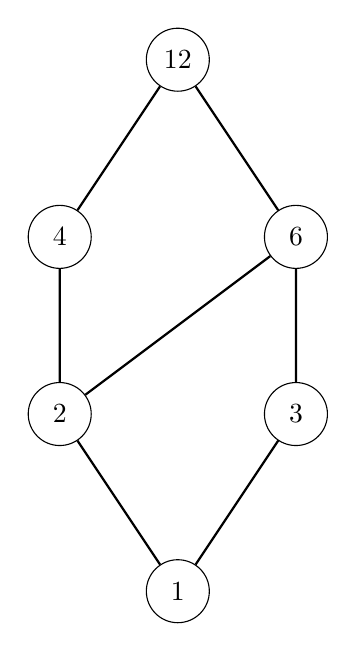
\begin{tikzpicture}[scale=1.5, every node/.style={circle, draw, minimum size=0.8cm, inner sep=0pt}]
        % Nodes
        \node (1) at (0,0) {1};
        \node (2) at (-1,1.5) {2};
        \node (3) at (1,1.5) {3};
        \node (4) at (-1,3) {4};
        \node (6) at (1,3) {6};
        \node (12) at (0,4.5) {12};
        
        % Edges
        \draw[thick] (1) -- (2);
        \draw[thick] (1) -- (3);
        \draw[thick] (2) -- (4);
        \draw[thick] (2) -- (6);
        \draw[thick] (3) -- (6);
        \draw[thick] (4) -- (12);
        \draw[thick] (6) -- (12);
    \end{tikzpicture}
\end{center}

\subsection{Example 2: The Subset Relation on a Power Set}
Consider the set $S = \{a, b, c\}$. Let the POSET be the power set of $S$, $\mathcal{P}(S)$, ordered by the subset relation $\subseteq$.
\vspace{0.5cm}
\begin{center}
    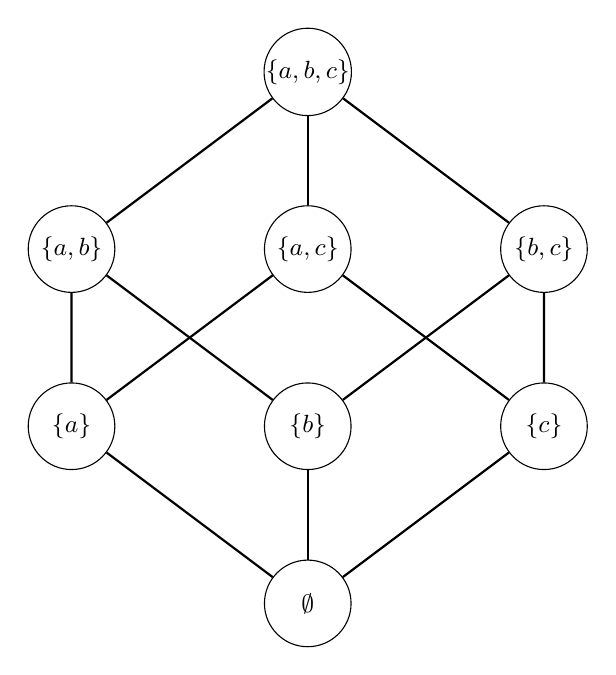
\begin{tikzpicture}[scale=1.5, every node/.style={circle, draw, minimum size=1.1cm, inner sep=0pt, font=\small}]
        % Nodes
        \node (empty) at (0,0) {$\emptyset$};
        \node (a) at (-2,1.5) {$\{a\}$};
        \node (b) at (0,1.5) {$\{b\}$};
        \node (c) at (2,1.5) {$\{c\}$};
        \node (ab) at (-2,3) {$\{a,b\}$};
        \node (ac) at (0,3) {$\{a,c\}$};
        \node (bc) at (2,3) {$\{b,c\}$};
        \node (abc) at (0,4.5) {$\{a,b,c\}$};
        
        % Edges
        \draw[thick] (empty) -- (a);
        \draw[thick] (empty) -- (b);
        \draw[thick] (empty) -- (c);
        \draw[thick] (a) -- (ab);
        \draw[thick] (a) -- (ac);
        \draw[thick] (b) -- (ab);
        \draw[thick] (b) -- (bc);
        \draw[thick] (c) -- (ac);
        \draw[thick] (c) -- (bc);
        \draw[thick] (ab) -- (abc);
        \draw[thick] (ac) -- (abc);
        \draw[thick] (bc) -- (abc);
    \end{tikzpicture}
\end{center}

\end{document}